\section{Application server}\label{sec:archserver}

The application server provides the management of the user interface for the web
client thanks to the use of servlets that exploit the JSP technology, and it
manages the business logic using the JakartaEE framework that allows it to
communicate with the Erlang subsystem. Furthermore, given the purpose of the
application, the application server implements an asynchronous communication
system with the web clients, which allows users to receive real-time updates on
the status of the auctions, using the WebSocket communication protocol.

\figref{fig:application-server-arch} shows the application server's
architecture.

\begin{figure}[htb]
	\centering
	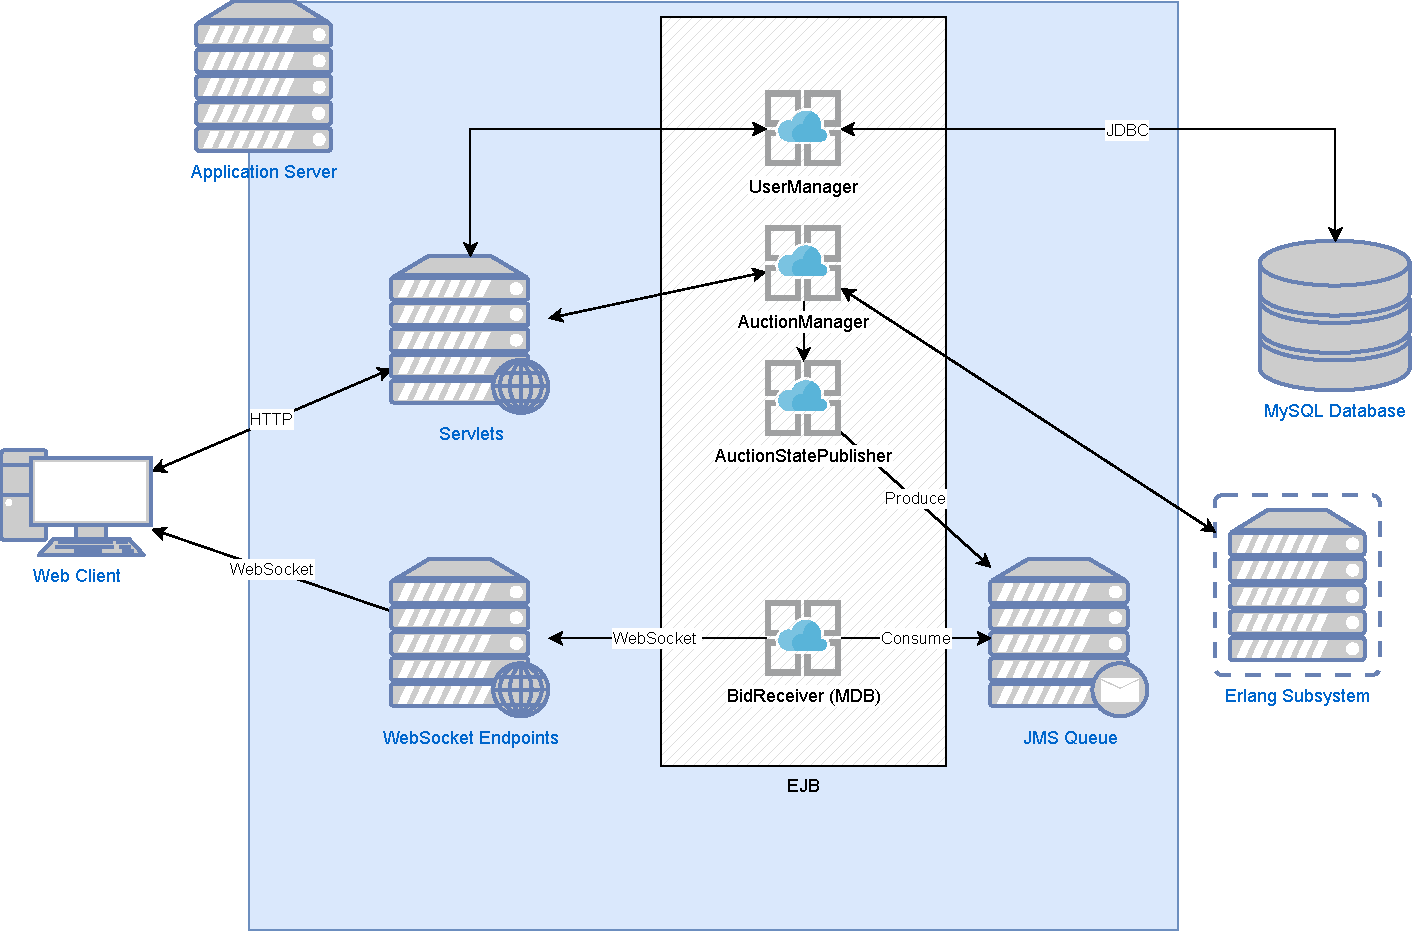
\includegraphics[width=\textwidth]{application-server-arch}
	\caption{Application Server
	architecture.}\label{fig:application-server-arch}
\end{figure}

\subsection{JEE Beans}

JEE Beans provide business logic interfaces implementation. They implement the
interface between MySQL database (for user data) and Erlang subsystem towards
servlets. It is composed of the following components:

\begin{description}
	\item[AuctionManager] A stateless session bean that manages the
		communication with the Erlang subsystem, exposing the interfaces
		between the former and servlets. This bean is also in charge of
		communicating changes in the auctions’ state from the Erlang
		subsystem to the \code{AuctionStatePublisher}.
	\item[UserManager] A stateless session bean that manages the
		communication with the MySQL database (that manages user
		informations), exposing the interfaces between the former and
		servlets.
	\item[AuctionStatePublisher] A singleton session bean that act as a
		proxy for the actual state of all the bids in the Erlang
		subsystem, whenever the state changes (because a bid has been
		made or deleted, or an auction is closed) this bean is informed
		from the \code{AuctionManager}. Furthermore, it acts as a
		producer for a JMS queue, to promptly notify clients on changes
		in the auction
\end{description}

\subsection{JMS and Message Driven Beans}

JMS and Message Driver Beans provide the messaging framework for bids
dispatching from Erlang subsystem for notifying changes in auctions’ state to
clients. It is composed of the following components:

\begin{description}
	\item[JMS Queue] a queue is used in order to asynchronously notify
		clients of changes in the auction state.
	\item[BidReceiver] Is a message-driven bean that receives the new state
		of the auctions from the queue and using WebSocket
		ClientEndpoint API initiates the communication towards a
		WebSocket ServerEndpoint. Then the ServerEndpoint communicate to
		the clients the updates.
\end{description}

\subsection{WebSocket}

It be used as communication protocol among JEE beans and web clients. The web
server acts as a relay, providing two endpoints: one from the application server
towards the web server, and the other from the web server towards the clients.

This protocol allows us to implement a real time notification broadcasting
service for all the clients interested in an auction in a clean way (no polling
is needed), giving us the possibility to initiate the communication from the
backend.
